
\begin{wrapfigure}{r}{0.35\textwidth}
  \begin{minipage}{\linewidth}
    \centering\captionsetup[subfigure]{justification=centering}
  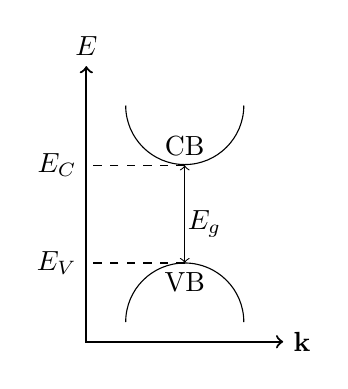
\begin{tikzpicture}[scale=1]
      \draw [<->,thick] (0,3.5) node (yaxis) [above] {$E$}
          |- (2.5,0) node (xaxis) [right] {$\textbf{k}$};
      \draw (0.5,0.25) arc(180:0:0.75cm);
      \draw (2.0,3.0) arc(0:-180:0.75cm);
      \coordinate (VB) at (1.25,1.0);
      \coordinate (CB) at (1.25,2.24);
      \draw[<->] (CB) node[above] {CB}
        -| (VB) node[below] {VB};
      \draw[dashed] (VB) -- (0,1.0) node[left]{$E_V$};
      \draw[dashed] (CB) -- (0,2.24) node[left]{$E_C$};
      \node at (1.5,1.5) {$E_g$};
  \end{tikzpicture}
  \subcaption{}
  \label{fig:directbandgap}
  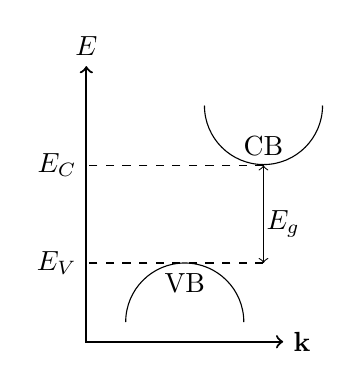
\begin{tikzpicture}[scale=1]
      \draw [<->,thick] (0,3.5) node (yaxis) [above] {$E$}
          |- (2.5,0) node (xaxis) [right] {$\textbf{k}$};
      \draw (0.5,0.25) arc(180:0:0.75cm);
      \draw (3.0,3.0) arc(0:-180:0.75cm);
      \coordinate (VB) at (2.25,1.0);
      \coordinate (CB) at (2.25,2.24);
      \draw[<->] (CB) node[above] {CB}
        -| (VB);
      \draw[dashed] (VB) -- (0,1.0) node[left]{$E_V$};
      \draw[dashed] (CB) -- (0,2.24) node[left]{$E_C$};
      \node at (2.5,1.5) {$E_g$};
      \node at (1.25,0.75) {VB};
  \end{tikzpicture}
  \label{fig:indirectbandgap}
  \subcaption{}
  \end{minipage}
  \caption{A schematic drawing of a (a) direct bandgap and an (b) indirect bandgap.}
\end{wrapfigure}
